\documentclass[12pt, a4paper, oneside, openright, titlepage]{book}
\usepackage[utf8]{inputenc}
\raggedbottom
\usepackage{import}


%%%%%%%%%%%%%%%%% Book Formatting Comments:

%%%%%%%%%%%%%%%%%%%%%%%%%%%%%%%%%%%%% for Part

%%%%%%%%%%%%%%%%%%%%%% for chapter

%%%%%%%%%%%%%%%%%%%% for section








%%%%%% PACKAGES %%%%%%%
\usepackage{hyperref}
\hypersetup{
    colorlinks,
    citecolor=black,
    filecolor=black,
    linkcolor=black,
    urlcolor=black
}
\usepackage{amsmath} % Math display options
\usepackage{amssymb} % Math symbols
\usepackage{amsfonts} % Math fonts
\usepackage{amsthm}
\usepackage{mathtools} % General math tools
\usepackage{array} % Allows you to write arrays
\usepackage{empheq} % For boxing equations
\usepackage{mathabx}
\usepackage{mathrsfs}
\usepackage{nameref}

\usepackage{soul}
\usepackage[normalem]{ulem}

\usepackage{txfonts}
\usepackage{cancel}
\usepackage[toc, page]{appendix}
\usepackage{titletoc,tocloft}
\setlength{\cftchapindent}{1em}
\setlength{\cftsecindent}{2em}
\setlength{\cftsubsecindent}{3em}
\setlength{\cftsubsubsecindent}{4em}
\usepackage{titlesec}

\titleformat{\section}
  {\normalfont\fontsize{25}{15}\bfseries}{\thesection}{1em}{}
\titleformat{\section}
  {\normalfont\fontsize{20}{15}\bfseries}{\thesubsection}{1em}{}
\setcounter{secnumdepth}{1}  
  
  

\newcommand\numberthis{\refstepcounter{equation}\tag{\theequation}} % For equation labelling
\usepackage[framemethod=tikz]{mdframed}

\usepackage{tikz} % For drawing commutative diagrams
\usetikzlibrary{cd}
\usetikzlibrary{calc}
\tikzset{every picture/.style={line width=0.75pt}} %set default line width to 0.75p

\usepackage{datetime}
\usepackage[margin=1in]{geometry}
\setlength{\parskip}{1em}
\usepackage{graphicx}
\usepackage{float}
\usepackage{fancyhdr}
\setlength{\headheight}{15pt} 
\pagestyle{fancy}
\lhead[\leftmark]{}
\rhead[]{\leftmark}

\usepackage{enumitem}

\usepackage{url}
\allowdisplaybreaks

%%%%%% ENVIRONMENTS %%%
\definecolor{purp}{rgb}{0.29, 0, 0.51}
\definecolor{bloo}{rgb}{0, 0.13, 0.80}



%%\newtheoremstyle{note}% hnamei
%{3pt}% hSpace above
%{3pt}% hSpace belowi
%{}% hBody fonti
%{}% hIndent amounti
%{\itshape}% hTheorem head fonti
%{:}% hPunctuation after theorem headi
%{.5em}% hSpace after theorem headi
%{}% hTheorem head spec (can be left empty, meaning ‘normal’)i


%%%%%%%%%%%%% THEOREM STYLES

\newtheoremstyle{BigTheorem}
{20pt}
{20pt}
{\slshape}
{}
{\Large\color{purp}\bfseries}
{.}
{\newline}
{\thmname{#1}\thmnumber{ #2}\thmnote{ (#3)}}



\newtheoremstyle{TheoremClassic}
{15pt}
{15pt}
{\slshape}
{}
{\bfseries}
{.}
{.5em}
{}

\newtheoremstyle{Definitions}
{15pt}
{15pt}
{\slshape}
{}
{\bfseries}
{.}
{.5em}
{\thmname{#1}\thmnumber{ #2}\thmnote{ (#3)}}


\newtheoremstyle{Remarks}
{10pt}
{10pt}
{\upshape}
{}
{\bfseries}
{.}
{.5em}
{}

\newtheoremstyle{Examples}
{10pt}
{10pt}
{\upshape}
{}
{\bfseries}
{.}
{.5em}
{}


%%%%%%%%%%%%% THEOREM DEFINITIONS

\theoremstyle{BigTheorem}
\newtheorem{namthm}{Theorem}
\newtheorem{conj}[namthm]{Conjecture}

\theoremstyle{TheoremClassic}
\newtheorem{thm}{Theorem}[section]
\newtheorem*{thm*}{Theorem}
\newtheorem{lem}[thm]{Lemma}
\newtheorem{cor}[thm]{Corollary}
\newtheorem{prop}[thm]{Proposition}
\newtheorem{claim}[thm]{Claim}


\theoremstyle{Definitions}
\newtheorem{defn}{Definition}[section]
\newtheorem{axi}[defn]{Axiom}
\newtheorem{cust}[defn]{}
\newtheorem{cons}[defn]{Construction}
\newtheorem{props}[defn]{Properties}
\newtheorem{proc}[defn]{Process}
\newtheorem*{law}{Law}


\theoremstyle{Examples}
\newtheorem{eg}{Example}[section]
\newtheorem{noneg}[eg]{Non-Example}
\newtheorem{xca}[eg]{Exercise}


\theoremstyle{Remarks}
\newtheorem{rmk}{Remark}[section]
\newtheorem{qst}[rmk]{Question}
\newtheorem*{ans}{Answer}
\newtheorem{obs}[rmk]{Observation}
\newtheorem{rec}[rmk]{Recall}
\newtheorem{summ}[rmk]{Summary}
\newtheorem{nota}[rmk]{Notation}
\newtheorem{note}[rmk]{Note}



\renewcommand{\qedsymbol}{$\blacksquare$}


\numberwithin{equation}{section}

\newenvironment{qest}{
    \begin{center}
        \em
    }
    {
    \end{center}
    }

%%%%%% MACROS %%%%%%%%%
%% New Commands
\newcommand{\ip}[1]{\langle#1\rangle} %%% Inner product
\newcommand{\abs}[1]{\lvert#1\rvert} %%% Modulus
\newcommand\diag{\operatorname{diag}} %%% diag matrix
\newcommand\tr{\mbox{tr}\.} %%% trace
\newcommand\C{\mathbb C} %%% Complex numbers
\newcommand\R{\mathbb R} %%% Real numbers
\newcommand\Z{\mathbb Z} %%% Integers
\newcommand\Q{\mathbb Q} %%% Rationals
\newcommand\N{\mathbb N} %%% Naturals
\newcommand\F{\mathbb F} %%% An arbitrary field
\newcommand\ste{\operatorname{St}} %%% Steinberg Representation
\newcommand\GL{\mathbf{GL}} %%% General Linear group
\newcommand\SL{\mathbf{SL}} %%% Special linear group
\newcommand\gl{\mathfrak{gl}} %%% General linear algebra
\newcommand\G{\mathbf{G}} %%% connected reductive group
\newcommand\g{\mathfrak{g}} %%% Lie algebra of G
\newcommand\Hbf{\mathbf{H}} %%% Theta fixed points of G
\newcommand\X{\mathbf{X}} %%% Symmetric space X
\newcommand{\catname}[1]{\normalfont\textbf{#1}}
\newcommand{\Set}{\catname{Set}} %%% Category set
\newcommand{\Grp}{\catname{Grp}} %%% Category group
\newcommand{\Rmod}{\catname{R-Mod}} %%% Category r-modules
\newcommand{\Mon}{\catname{Mon}} %%% Category monoid
\newcommand{\Ring}{\catname{Ring}} %%% Category ring
\newcommand{\Topp}{\catname{Top}} %%% Category Topological spaces
\newcommand{\Vect}{\catname{Vect}_{k}} %%% category vector spaces'
\newcommand\Hom{\mathbf{Hom}} %%% Arrows

\newcommand{\map}[2]{\begin{array}{c} #1 \\ #2 \end{array}}

\newcommand{\Emph}[1]{\textbf{\ul{\emph{#1}}}}

\newcommand{\mapsfrom}{\mathrel{\reflectbox{\ensuremath{\mapsto}}}}


%% Math operators
\DeclareMathOperator{\ran}{Im} %%% image
\DeclareMathOperator{\aut}{Aut} %%% Automorphisms
\DeclareMathOperator{\spn}{span} %%% span
\DeclareMathOperator{\ann}{Ann} %%% annihilator
\DeclareMathOperator{\rank}{rank} %%% Rank
\DeclareMathOperator{\ch}{char} %%% characteristic
\DeclareMathOperator{\ev}{\bf{ev}} %%% evaluation
\DeclareMathOperator{\sgn}{sign} %%% sign
\DeclareMathOperator{\id}{Id} %%% identity
\DeclareMathOperator{\supp}{Supp} %%% support
\DeclareMathOperator{\inn}{Inn} %%% Inner aut
\DeclareMathOperator{\en}{End} %%% Endomorphisms
\DeclareMathOperator{\sym}{Sym} %%% Group of symmetries


%% Diagram Environments
\iffalse
\begin{center}
    \begin{tikzpicture}[baseline= (a).base]
        \node[scale=1] (a) at (0,0){
          \begin{tikzcd}
           
          \end{tikzcd}
        };
    \end{tikzpicture}
\end{center}
\fi




\newdateformat{monthdayyeardate}{%
    \monthname[\THEMONTH]~\THEDAY, \THEYEAR}
%%%%%%%%%%%%%%%%%%%%%%%

%%% Specific Macros %%%


%%%%%% BEGIN %%%%%%%%%%


\begin{document}

%%%%%% TITLE PAGE %%%%%

\begin{titlepage}
    \centering
    \scshape
    \vspace*{\baselineskip}
    \rule{\textwidth}{1.6pt}\vspace*{-\baselineskip}\vspace*{2pt}
    \rule{\textwidth}{0.4pt}
    
    \vspace{0.75\baselineskip}
    
    {\LARGE Mathematical Physics: A Complete Guide}
    
    \vspace{0.75\baselineskip}
    
    \rule{\textwidth}{0.4pt}\vspace*{-\baselineskip}\vspace{3.2pt}
    \rule{\textwidth}{1.6pt}
    
    \vspace{2\baselineskip}
    Phys 435 \\
    \vspace*{3\baselineskip}
    \monthdayyeardate\today \\
    \vspace*{5.0\baselineskip}
    
    {\scshape\Large Elijah Thompson, \\ Physics and Math Honors\\}
    
    \vspace{1.0\baselineskip}
    \textit{Solo Pursuit of Learning}
    \vfill
    \enlargethispage{1in}
    \begin{figure}[b!]
    \makebox[\textwidth]{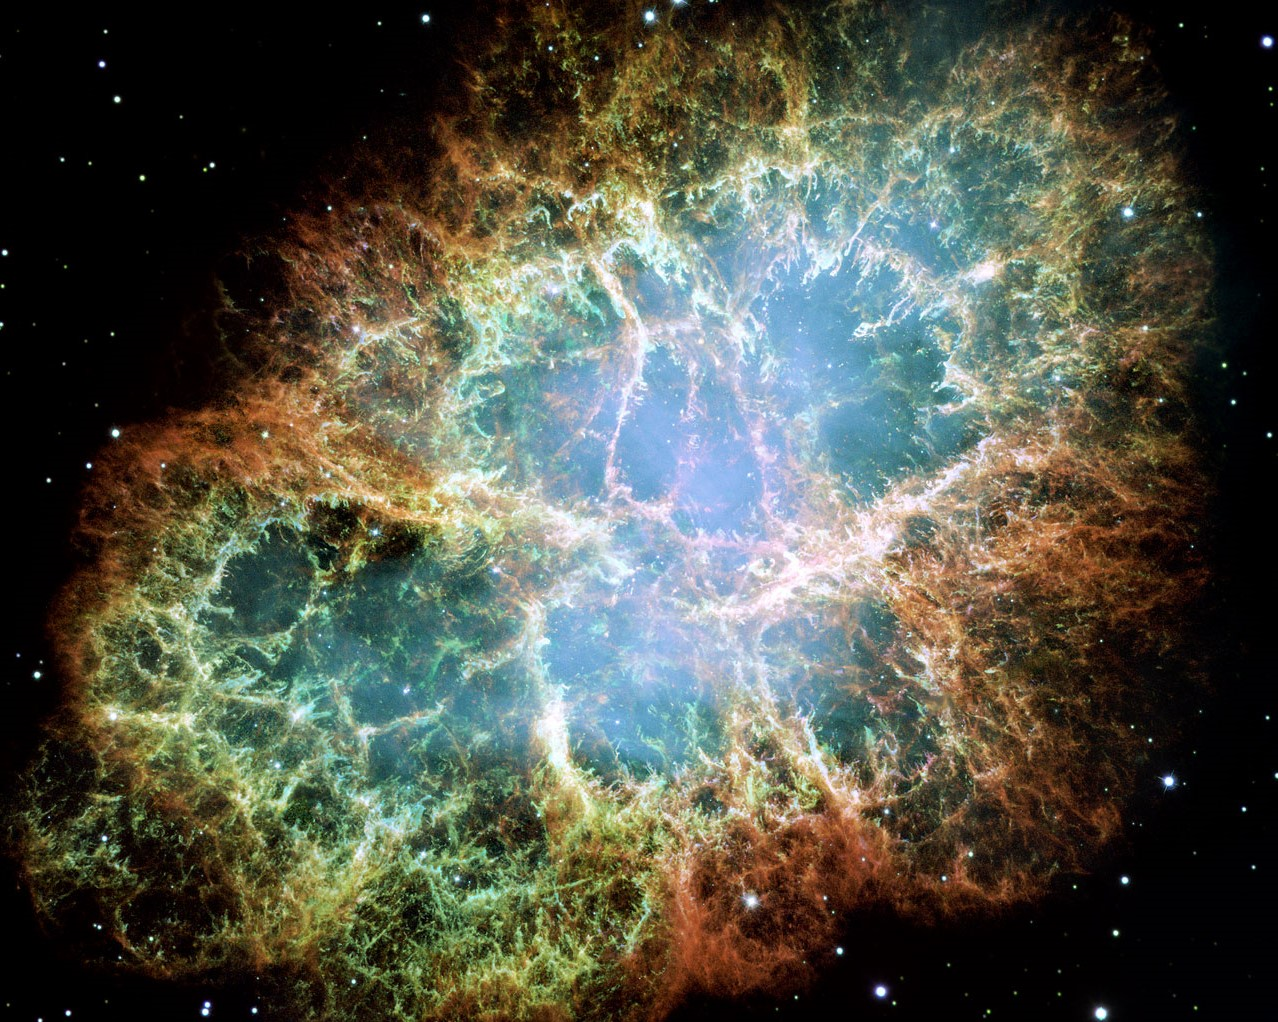
\includegraphics[width=\paperwidth, height =10cm]{../Crab.jpg}}
    \end{figure}
\end{titlepage}

%%%%%%%%%%%%%%%%%%%%%%%
\tableofcontents



%%%%%%%%%%%%%%%%%%%%%%%%%%%%%%%%%%%%% Part 1
\part{Complex Analysis}


%%%%%%%%%%%%%%%%%%%%%% Chapter 1.1
\chapter{Properties of Complex Functions}

%%%%%%%%%%%%%%%%%%%% Section 1.1.1
\section{Elementary Definitions}

Complex functions are functions $f:D\subseteq \C\rightarrow \C$ of the form $f(z) = u(z) + iv(z)$, where $u$ and $v$ are real valued functions.

\begin{defn}
    A complex valued function $f(z)$ is \Emph{complex differentiable} at a point $z_0$ in its domain if the limit \begin{equation*}
        f'(z_0) = \lim\limits_{z\rightarrow z_0}\left[\frac{f(z)-f(z_0)}{z-z_0}\right]
    \end{equation*}
    exists.
\end{defn}

\begin{defn}
    A function that is single-valued and differentiable at all points of a domain $D$ is said to be \Emph{analytic} in $D$.
\end{defn}




%%%%%%%%%%%%%%%%%%%% Section 1.1.2
\section{Multivalued Functions and Branch Cuts}


%%%%%%%%%%%%%%%%%%%% Section 1.1.3
\section{Analytic Functions and the Cauchy-Riemann Equations}

For a complex-valued function $f(z) = u(z)+iv(z)$ to be complex differentiable on a domain $D$, it is necessary that $u$ and $v$ satisfy the \Emph{Cauchy-Riemann} equations \begin{equation*}
    \frac{\partial u}{\partial x} = \frac{\partial v}{\partial y},\;\;\text{ and }\;\;\frac{\partial v}{\partial x} = -\frac{\partial u}{\partial y}
\end{equation*}

Further, given that $f(z)$ is complex differentiable we have that \begin{equation*}
    f'(z) = \frac{\partial f}{\partial x} = -i\frac{\partial f}{\partial y}
\end{equation*}

\begin{thm}
    If $f(z) = u+iv$ is a real-continuously differentiable function of $x,y$ as viewed as a function $f:\R^2\rightarrow \R^2$, and $u$ and $v$ satisfy the Cauchy-Riemann equations on some domain $D$, then $f(z)$ is analytic on $D$.
\end{thm}

Define the complex differential operators \begin{equation*}
    \frac{\partial}{\partial z} = \frac{\partial x}{\partial z}\frac{\partial }{\partial x}+\frac{\partial y}{\partial z}\frac{\partial }{\partial y} = \frac{1}{2}\left[\frac{\partial}{\partial x}-i\frac{\partial}{\partial y}\right]
\end{equation*}
and \begin{equation*}
    \frac{\partial}{\partial \overline{z}} = \frac{\partial x}{\partial \overline{z}}\frac{\partial }{\partial x}+\frac{\partial y}{\partial \overline{z}}\frac{\partial }{\partial y} = \frac{1}{2}\left[\frac{\partial}{\partial x}+i\frac{\partial}{\partial y}\right]
\end{equation*}
using the relations $x = (z+\overline{z})/2$ and $y = -i(z-\overline{z})/2$. Then we have that \begin{equation*}
    \frac{\partial f}{\partial z} = \frac{1}{2}\left[\frac{\partial f}{\partial x}-i\frac{\partial f}{\partial y}\right] = f'(z)
\end{equation*}
provided $f$ is holomorphic, and \begin{equation*}
    \frac{\partial f}{\partial \overline{z}} = \frac{1}{2}\left[\frac{\partial f}{\partial x}+i\frac{\partial f}{\partial y}\right] = \frac{1}{2}\left[(u_x+iv_x) + i(u_y+iv_y)\right] = \frac{1}{2}\left[(u_x-v_y)+i(u_y+v_x)\right]
\end{equation*}
which is zero if and only if $f$ satisfies the Cauchy-Riemann equations. This implies that if $f$ is analytic on a domain, then it cannot be a function of $\overline{z}$ on that domain.

\begin{thm}
    If $f(z)= u(z)+iv(z)$ is holomorphic and twice continuously differentiable on some domain, then $u$ and $v$ are harmonic on that domain.
\end{thm}
\begin{proof}
    Observe that $u_{xx} = v_{yx} = v_{xy} = -u_{yy}$, so $u_{xx} + u_{yy} = 0$ and we conclude that $\Delta u = 0$. Similarly, $\Delta v = 0$, so both functions are harmonic.
\end{proof}

We now observe that if $f(z) = u(z)+iv(z)$ is complex differentiable, then the curves $u(z) = C_1$ and $v(z) = C_2$, if they intersect, intersect at right angles. Indeed, \begin{align*}
    \nabla u\cdot \nabla v = u_xv_x+u_yv_y = -u_xu_y+u_yu_x = 0
\end{align*}
using the Cauchy-Riemann relations.




%%%%%%%%%%%%%%%%%%%% Section 1.1.4
\section{Singularities and Zeros}


%%%%%%%%%%%%%%%%%%%% Section 1.1.5
\section{Conformal Mappings}


%%%%%%%%%%%%%%%%%%%%%% Chapter 1.2
\chapter{Power Series and Laurent Series}


%%%%%%%%%%%%%%%%%%%% Section 1.2.1
\section{Power Series Fundamentals}


\begin{defn}
    A complex power series about a point $z_0$ is a series of a complex variable $z$, such that \begin{equation*}
        f(z) = \sum_{n=0}^{\infty}a_n(z-z_0)^n
    \end{equation*}
    In modulus form, $z = z_0+r^ne^{i\theta}$, we have \begin{equation*}
        f(z) = \sum_{n=0}^{\infty}a_nr^ne^{in\theta}
    \end{equation*}
\end{defn}

\begin{defn}
    We say that the series \begin{equation*}
        f(z) = \sum_{n=0}^{\infty}a_nr^ne^{in\theta}
    \end{equation*}
    is absolutely convergent if \begin{equation*}
        \sum_{n=0}^{\infty}|a_n|r^n
    \end{equation*}
    is convergent.
\end{defn}

\begin{thm}
    If we have a complex series of the form \begin{equation*}
        f(z) = \sum_{n=0}^{\infty}a_nr^ne^{in\theta}
    \end{equation*}
    then the radius of convergence of the series is given by \begin{equation*}
        R = \frac{1}{\lim\limits_{n\rightarrow \infty}\sqrt[n]{|a_n|}}
    \end{equation*}
    or equivalently \begin{equation*}
        R = \lim\limits_{n\rightarrow \infty}\left|\frac{a_n}{a_{n+1}}\right|
    \end{equation*}
    Further, for $|z| < R$, the series converges normally (i.e. $\sum_{n=0}^{\infty}a_n||z-z_0||_R^n$ converges), and hence both absolutely and uniformly.
\end{thm}

\begin{thm}
    $f(z)$ is holomorphic for $|z-z_0| < \rho$ if and only if $f(z)$ has power series representation \begin{equation*}
        f(z) = \sum_{n=0}^{\infty}a_n(z-z_0)^n,\;\;\;|z-z_0| < \rho
    \end{equation*}
    where \begin{equation*}
        a_n = \frac{f^{(n)}(z_0)}{n!},\;\;n\geq 0
    \end{equation*}
    and where the power series has radius of convergence $R \geq \rho$. For any fixed $r$, $0 < r < \rho$, we also have \begin{equation*}
        a_n = \frac{1}{2\pi i}\oint_{|w-z_0| = r}\frac{f(w)}{(w-z_0)^{n+1}}dw,\;\;\;n\geq 0
    \end{equation*}
    Additionally, the derivatives of $f(z)$ are obtained by term-by-term differentiation \begin{equation*}
        f^{(m)}(z) = \sum_{n=m}^{\infty}\frac{n!}{(n-m)!}a_n(z-z_0)^{n-m}
    \end{equation*}
\end{thm}











%%%%%%%%%%%%%%%%%%%% Section 1.2.2
\section{Laurent Series}


%%%%%%%%%%%%%%%%%%%% Section 1.2.3
\section{Series Operations}



%%%%%%%%%%%%%%%%%%%%%% Chapter 1.3
\chapter{Complex Integration}

%%%%%%%%%%%%%%%%%%%% Section 1.3.1
\section{Complex Integral}


%%%%%%%%%%%%%%%%%%%% Section 1.3.2
\section{Cauchy's Theorems}


%%%%%%%%%%%%%%%%%%%% Section 1.3.3
\section{Residue Theorem}


%%%%%%%%%%%%%%%%%%%% Section 1.3.4
\section{Contour Integrals}


%%%%%%%%%%%%%%%%%%%%%% Chapter 1.4
\chapter{Applications of Complex Functions}


%%%%%%%%%%%%%%%%%%%% Section 1.4.1
\section{Complex Potentials}


%%%%%%%%%%%%%%%%%%%% Section 1.4.2
\section{Finding Zeros}


%%%%%%%%%%%%%%%%%%%% Section 1.4.3
\section{Inverse Laplace}

%%%%%%%%%%%%%%%%%%%% Section 1.4.4
\section{Stokes' Equations and Airy Integrals}


%%%%%%%%%%%%%%%%%%%% Section 1.4.5
\section{WKB Methods, and Integral Approximations}




%%%%%%%%%%%%%%%%%%%%%%%%%%%%%%%%%%%%% Part 2
\part{PDEs}


%%%%%%%%%%%%%%%%%%%%%% Chapter 2.1
\chapter{General and Particular Solutions}

%%%%%%%%%%%%%%%%%%%% Section 2.1.1
\section{Important Examples and Motivation}



%%%%%%%%%%%%%%%%%%%% Section 2.1.2
\section{General Forms of Solutions}



%%%%%%%%%%%%%%%%%%%% Section 2.1.3
\section{Wave and Diffusion Equations}



%%%%%%%%%%%%%%%%%%%% Section 2.1.4
\section{Existence and Uniqueness}




%%%%%%%%%%%%%%%%%%%%%% Chapter 2.2
\chapter{Fourier Series}


%%%%%%%%%%%%%%%%%%%% Section 2.2.1
\section{Initial Definitions and Dirichlet Conditions}


\begin{defn}
    Sufficients conditions for which a function $f(x)$ to have its Fourier series to converge to it are known as the \Emph{Dirichlet conditions}: \begin{enumerate}
        \item[(i)] $f(x)$ must be periodic; i.e. there exists $p \in \R$ such that $f(x+p) = f(x)$ for all $x \in \R$.
        \item[(ii)] $f(x)$ must be continuous, except possibly at a finite number of jump (i.e. finite) discontinuities in any bounded interval.
        \item[(iii)] $f(x)$ must be of \Emph{bounded variation} on any bounded interval, which is to say its total variation is finite; if $f$ is differentiable and its derivative is Riemann-integrable on the interval, then the total variation is the absolute integral of the derivative over the interval: $$V_a^b(f) = \int_a^b|f'(x)|dx$$
            An alternative formulation is to require that any bounded interval contains only a finite number of extrema of $f$.
        \item[(iv)] $f(x)$ is absolutely integrable over a period, so $$\int_0^p|f(x)|dx < \infty$$
    \end{enumerate}
    If these criterions hold, the Fourier series converges to $f(x)$ at all points where the function is continuous.
\end{defn}

Recall that a function $f(x)$ can be split into an even and odd part: \begin{equation*}
    f(x) = \frac{1}{2}[f(x) + f(-x)] + \frac{1}{2}[f(x) - f(-x)] = f_{even}(x) + f_{odd}(x)
\end{equation*}
Then, we can write the even component as a cosine series and the odd component as a sine series.

\begin{prop}
    For any $L \in \R$, the set of functions \begin{equation*}
        \left\{1,\cos\frac{2\pi x}{L},\sin\frac{2\pi x}{L},\cos\frac{2\pi 2x}{L},\sin\frac{2\pi 2x}{L},...,\cos\frac{2\pi nx}{L},\sin\frac{2\pi nx}{L},...\right\}
    \end{equation*}
    form an orthogonal set with respect to the inner product \begin{equation*}
        \langle f,g\rangle = \int_{x_0}^{x_0+L}f(x)g(x)dx
    \end{equation*}
    for $x_0 \in \R$ fixed. In particular, we have \begin{align*}
        \int_{x_0}^{x_0+L}\sin\frac{2\pi nx}{L}\cos\frac{2\pi mx}{L}dx &= 0,\;\;\forall n,m \in \N\cup \{0\} \\
        \int_{x_0}^{x_0+L}\cos\frac{2\pi nx}{L}\cos\frac{2\pi mx}{L}dx &= \left\{\begin{array}{lc} L & \text{if } n = m = 0, \\ \frac{L}{2} & \text{if } n = m > 0, \\ 0 & \text{if } n \neq m \end{array}\right. \\
        \int_{x_0}^{x_0+L}\sin\frac{2\pi nx}{L}\sin\frac{2\pi mx}{L}dx &= \left\{\begin{array}{lc} 0 & \text{if } n = m = 0, \\ \frac{L}{2} & \text{if } n = m > 0, \\ 0 & \text{if } n \neq m \end{array}\right. \\
    \end{align*}
\end{prop}


\begin{defn}
    The classical Fourier series expansion of a function $f(x)$ is \begin{equation}
        f(x) \sim \frac{a_0}{2} + \sum_{n=1}^{\infty}\left[a_n\cos\frac{2\pi xn}{L}+b_n\sin\frac{2\pi nx}{L}\right]
    \end{equation}
    where $a_0,a_n,b_n$, for $n \geq 1$, are called the \Emph{Fourier coefficients}
\end{defn}

For a periodic function $f(x)$ of period $L$, we use the orthogonality conditions to find the Fourier coefficients as follows: \begin{align}
    a_0 &= \frac{2}{L}\int_{x_0}^{x_0+L}f(x)\cdot 1dx \\
    a_n &= \frac{2}{L}\int_{x_0}^{x_0+L}f(x)\cdot \cos\frac{2\pi nx}{L}dx \\
    b_n &= \frac{2}{L}\int_{x_0}^{x_0+L}f(x)\cdot \sin\frac{2\pi nx}{L}dx
\end{align}
where $x_0$ is arbitrary, but fixed, and $n \geq 1$.


\subsection{Symmetry Conditions}

From these coefficient equations we observe that if $f(x)$ is even with respect to the origin then all sine terms, $b_n$, are zero. Conversely, if $f(x)$ is odd with respect to the origin then all cosine terms, $a_n$, are zero. We now consider a more subtle symmetry about $L/4$, where $L$ is a period of $f$, so $f(x+L) = f(x)$ for all $x \in \R$.

\begin{defn}
    We say that $f(x)$ has even symmetry about $L/4$ if $f(L/4-x) = f(x-L/4)$ for all $x \in \R$. We say that $f(x)$ has odd symmetry about $L/4$ if $f(L/4-x) = -f(x-L/4)$.
\end{defn}

We consider the sine terms of $g(x) = f(x-L/4)$, and substitute $s = x-L/4$: \begin{align*}
    b_n &= \frac{2}{L}\int_{x_0}^{x_0+L}f(x-L/4)\sin\frac{2\pi nx}{L}dx \\
    &= \frac{2}{L}\int_{x_0-L/4}^{x_0-L/4+L}f(s)\sin\left[\frac{2\pi ns}{L} + \frac{\pi n}{2}\right]ds \\
    &= \frac{2}{L}\int_{x_0}^{x_0+L}f(s)\sin\left[\frac{2\pi ns}{L} + \frac{\pi n}{2}\right]ds
\end{align*}
where the limits of integration can be changed since $f$ is periodic. We observe that \begin{equation*}
    \sin\left[\frac{2\pi ns}{L} + \frac{\pi n}{2}\right] = \sin\frac{2\pi ns}{L}\cos\frac{\pi n}{2}+\cos\frac{2\pi ns}{L}\sin\frac{\pi n}{2}
\end{equation*}
so the trigonometric portion of the integrand is odd if $n$ is even and even if $n$ is odd. Then if $f(s)$ is even and $n$ is even the integral is zero, and similarly if $f(s)$ is odd and $n$ is odd the integral is zero. For the cosine coefficients we have \begin{equation*}
    \cos\left[\frac{2\pi ns}{L} + \frac{\pi n}{2}\right] = \cos\frac{2\pi ns}{L}\cos\frac{\pi n}{2}-\sin\frac{2\pi ns}{L}\sin\frac{\pi n}{2}
\end{equation*}
which is even if $n$ is even and odd if $n$ is odd. Then if $f(s)$ is even and $n$ is odd, the terms $a_n$ are zero, and if $f(s)$ is odd and $n$ is even, the terms $a_n$ are zero. In summary: \begin{itemize}
    \item If $f(x)$ is even about $L/4$, then $a_{2n-1} = 0$ and $b_{2n} = 0$ for all $n \geq 1$,
    \item If $f(x)$ is odd about $L/4$, then $a_{2n} = 0$ and $b_{2n+1} = 0$ for all $n \geq 0$.
\end{itemize}


%%%%%%%%%%%%%%%%%%%% Section 2.2.3
\section{Discontinuous and Non-Periodic Functions}

\subsection{Discontinuities}

\begin{defn}
    The error term for the Fourier series representation of $f$ when expressed as a partial sum with highest term $N$ is \begin{equation*}
        E_N(x) = \left|f(x) - \left[\frac{a_0}{2}+\sum_{n=1}^N\left(a_n\cos\frac{2\pi nx}{L}+b_n\sin\frac{2\pi nx}{L}\right)\right]\right|
    \end{equation*}
\end{defn}

If $f(x)$ is discontinuous at a point $a$ in the domain of interest, then the Fourier series for $f(x)$ does not produce a discontinuity at $a$ but rather converges to the value \begin{equation*}
    \frac{1}{2}[f(a+)+f(a-)]
\end{equation*}
where $f(a+) = \lim\limits_{x\rightarrow a^+}f(x)$ is the one-sided limit from above, and $f(a-) = \lim\limits_{x\rightarrow a^-}f(x)$ is the one-sided limit from below. Then, there exists sequences $u_n$ and $v_n$ such that $u_n,v_n\rightarrow a$, with $u_n < a$ for all $n$ and $v_n > a$ for all $n$ and \begin{equation*}
    E_N(u_N) \approx 0.9|f(a-)-f(a+)|\;\;\;E_N(v_N) \approx 0.9|f(a-)-f(a+)|
\end{equation*}
so the maximum value of the error $E_N(x)$ near $a$ does not approach zero as $N\rightarrow \infty$, but rather occurs closer and closer to $a$, and is essentially independent of $N$. This is known as the \Emph{Gibbs' phenomenon}.


\subsection{Non-Periodic Functions}

We often wish to analysize non-periodic functions using Fourier analysis, and this can be done by using appropriate periodic extensions:

\begin{thm}
    Suppose $h$ is differentiable on $[0,L]$; that is, $h'(x)$ exists for $0 < x< L$, and the one-sided derivatives \begin{equation*}
        h'_+ = \lim\limits_{x\rightarrow 0^+}\frac{h(x)-h(0)}{x}\;\;\text{ and }\;\;h'_-(L) = \lim\limits_{x\rightarrow L^-}\frac{h(x) - h(L)}{x-L}
    \end{equation*}
    both exist. \begin{itemize}
        \item Let $O$ denote the odd periodic extension of $h$ to $(-\infty,\infty)$ defined by \begin{equation*}
                O(x) = \left\{\begin{array}{lc} h(x), & 0 \leq x \leq L \\ -h(-x), & -L < x < 0,\end{array}\right.\text{ and } O(x+2L) = O(x),\;\;\forall x \in \R
        \end{equation*}
            Then $O$ is differentiable on $(-\infty,\infty)$ if and only if \begin{equation*}
                h(0) = h(L) = 0
            \end{equation*}
        \item Let $E$ denote the even periodic extension of $h$ to $(-\infty, \infty)$, defined by \begin{equation*}
                E(x) = \left\{\begin{array}{lc} h(x), & 0 \leq x \leq L \\ h(-x), & -L < x < 0,\end{array}\right.\text{ and } E(x+2L) = E(x),\;\;\forall x \in \R
        \end{equation*}
            Then $E$ is differentiable on $(-\infty,\infty)$ if and only if \begin{equation*}
                h_+'(0) = h_-'(L) = 0
            \end{equation*}
    \end{itemize}
\end{thm}





%%%%%%%%%%%%%%%%%%%% Section 2.2.4
\section{Integration and Differentiation}

\begin{thm}
    If $f(x)$ satisfies the Dirichlet conditions, then integrating the Fourier series of $f(x)$ term by term produces a Fourier series which converges to the integral of $f(x)$, modulo an arbitrary constant.
\end{thm}

\begin{thm}
    If $f(x)$ satisfies the Dirichlet conditions, is differentiable, and $f'(x)$ satisfies the Dirichlet conditions, then the Fourier series obtained by differentiating $f$'s Fourier series term by term converges to $f'(x)$.
\end{thm}

For general functional series we have the following important result: 

\begin{thm}
    A convergent infinite series \begin{equation*}
        W(z) = \sum_{n=1}^{\infty}w_n(z)
    \end{equation*}
    can be differentiated term by term on a closed interval $[z_1,z_2]$ to obtain \begin{equation*}
        W'(z) = \sum_{n=1}^{\infty}w'_n(z)
    \end{equation*}
    provided that $w'_n$ is continuous on $[z_1,z_2]$ and there exists a sequence $M_n$ of constants such that $\sum_{n=1}^{\infty}M_n$ converges and \begin{equation*}
        |w'_n(z)| \leq M_n,\;\;z_1 \leq z \leq z_2,\;\;n=1,2,3,...
    \end{equation*}
\end{thm}


%%%%%%%%%%%%%%%%%%%% Section 2.2.5
\section{Complex Fourier Series}

Recall that by DeMoivre's Formula we have the following for the complex exponential: \begin{equation*}
    \exp\left\{ix\right\} = \cos x + i\sin x
\end{equation*}
\begin{defn}
    For a function $f(x)$ of period $L$, its complex Fourier series expansion is given by \begin{equation*}
        f(x) \sim \sum_{n=-\infty}^{\infty}c_n\exp\left\{\frac{2\pi inx}{L}\right\}
    \end{equation*}
\end{defn}

We remark that the set of functions $$\left\{1,\exp\left\{\frac{2\pi x}{L}\right\},\exp\left\{\frac{2\pi 2x}{L}\right\},...\exp\left\{\frac{2\pi nx}{L}\right\},...\right\}$$
forms an orthogonal set under the complex inner product \begin{equation*}
    \langle f, g\rangle = \int_{x_0}^{x_0+L}f(x)\overline{g(x)}dx
\end{equation*}
for $x_0$ fixed with the relation \begin{equation*}
    \int_{x_0}^{x_0+L}\exp\left\{\frac{2\pi inx}{L}\right\}\exp\left\{-\frac{2\pi imx}{L}\right\}dx = \left\{\begin{array}{lc} L & \text{if } m = n \\ 0 & \text{if } m \neq n\end{array}\right.
\end{equation*} 
Then the Fourier coefficients are given by \begin{equation}
    c_n = \frac{1}{L}\int_{x_0}^{x_0+L}f(x)\exp\left\{-\frac{2\pi inx}{L}\right\}dx
\end{equation}

We expand the complex exponential in the Fourier series as follows: \begin{align*}
    \sum_{n=-\infty}^{\infty}c_n\exp\left\{\frac{2\pi nx}{L}\right\} &= \sum_{n=1}^{\infty}c_{-n}\exp\left\{\frac{-2\pi nx}{L}\right\} + c_0 + \sum_{n=1}^{\infty}c_n\exp\left\{\frac{2\pi nx}{L}\right\} \\
    &= c_0 + \sum_{n=1}^{\infty}\left[c_{-n}\left(\cos\frac{2\pi nx}{L} - i\sin\frac{2\pi nx}{L}\right) + c_n\left(\cos\frac{2\pi nx}{L} - i\sin\frac{2\pi nx}{L}\right)\right] \\
    &= c_0 + \sum_{n=1}^{\infty}\left[(c_{-n}+c_n)\cos\frac{2\pi nx}{L}+(ic_n - ic_{-n})\sin\frac{2\pi nx}{L}\right]
\end{align*}
From this expansion we find that \begin{align*}
    c_0 &= \frac{a_0}{2} \\
    c_{-n}+c_n &= a_n \\
    ic_n - ic_{-n} &= b_n
\end{align*}
for $n \geq 1$. Then we have that \begin{equation*}
    c_n = \frac{1}{2}(a_n - ib_n) \;\;\text{ and }\;\;c_{-n} = \frac{1}{2}(a_n + ib_n)
\end{equation*}
It follows that if $f(x)$ is real, so $a_n$ and $b_n$ are real, $c_{-n} = \overline{c_n}$.


\subsection{Parseval's Theorem}

\begin{namthm}[Parseval's Theorem]
    Suppose that $A(x)$ and $B(x)$ are two complex valued functions on $\R$ of period $2L$ that are square integrable with respect to the Lebesgue measure over intervals of period length with complex Fourier series\begin{equation*}
        A(x) = \sum_{n=-\infty}^{\infty}a_n\exp\left\{\frac{i\pi nx}{L}\right\},\;\text{ and }\;B(x) = \sum_{n=-\infty}^{\infty}b_n\exp\left\{\frac{i\pi nx}{L}\right\}
    \end{equation*}
    Then \begin{equation}
        \sum_{n=-\infty}^{\infty}a_n\overline{b_n} = \frac{1}{2L}\int_{-L}^LA(x)\overline{B(x)}dx
    \end{equation}
\end{namthm}
\begin{proof}
    Suppose $A(x)$ and $B(x)$ are as above, with corresponding Fourier series, and observe that \begin{align*}
        \frac{1}{2L}\int_{-L}^LA(x)\overline{B(x)}dx &= \sum_{n=-\infty}^{\infty}a_n\frac{1}{2L}\int_{-L}^L\overline{B(x)}\exp\left\{\frac{2\pi inx}{2L}\right\}dx \\
        &= \sum_{n=-\infty}^{\infty}a_n\overline{\left[\frac{1}{2L}\int_{-L}^LB(x)\exp\left\{\frac{-2\pi inx}{2L}\right\}dx\right]} \\
        &= \sum_{n=-\infty}^{\infty}a_n\overline{b_n}
    \end{align*}
    as desired.
\end{proof}

As a corollary, we have that for any function $f(x)$ of period $L$, \begin{equation*}
    \frac{1}{L}\int_{x_0}^{x_0+L}|f(x)|^2dx = \sum_{n=-\infty}^{\infty}|c_n|^2 = \frac{|a_0|^2}{4} + \frac{1}{2}\sum_{n=1}^{\infty}(a_n^2+b_n^2)
\end{equation*}

This says that the sum of the moduli squared of the complex Fourier coefficients is equal to the average value of $|f(x)|^2$ over one period. 



%%%%%%%%%%%%%%%%%%%%%% Chapter 2.3
\chapter{Integral Transforms}


%%%%%%%%%%%%%%%%%%%% Section 2.3.1
\section{Fourier Transform}


\subsection{Construction and Definitions}

Let $f(x)$ be defined on $-\infty < x < \infty$ such that it satisfies the Dirichlet conditions on $-L < x < L$. Then recall it has complex Fourier series expansion \begin{equation*}
    f(x) = \sum_{n=-\infty}^{\infty}c_n\exp\left\{\frac{in\pi x}{L}\right\}dx
\end{equation*}
with coefficients given by \begin{equation*}
    c_n = \frac{1}{2L}\int_{-L}^Lf(x)\exp\left\{\frac{-in\pi x}{L}\right\}dx
\end{equation*}
We now define \begin{equation*}
    \mu_n = \frac{n\pi}{L},\;\;\;n=0,\pm1,\pm2,...
\end{equation*}
so we have \begin{equation*}
    \Delta \mu_n = \mu_{n+1}-\mu_n = \frac{\pi}{L}
\end{equation*}
Note here we are constructin $f$ with period $2L$. Then the coefficients can be rewritten as \begin{equation*}
    c_n = \frac{\Delta\mu_n}{2\pi}\int_{-L}^Lf(x)\exp\left\{-i\mu_nx\right\}dx
\end{equation*}
and we define \begin{equation*}
    F_L(\mu) = \frac{1}{2\pi}\int_{-L}^Lf(x)\exp\left\{-i\mu x\right\}dx
\end{equation*}
so we can write the series as \begin{equation*}
    f(x) = \sum_{n=-\infty}^{\infty}F_L(\mu_n)\exp\left\{i\mu_nx\right\}\Delta \mu_n,\;\text{ and }\;c_n = F_L(\mu_n)\Delta \mu_n
\end{equation*}
In this form we take the limit as $L\rightarrow \infty$, which gives us the Riemann-integral \begin{equation}
    \boxed{f(x) = \int_{-\infty}^{\infty}F(\mu)\exp\left\{i\mu x\right\}dx}
\end{equation}
and \begin{equation}
    \boxed{F(\mu) = \frac{1}{2\pi}\int_{-\infty}^{\infty}f(x)\exp\left\{-i\mu x\right\}dx}
\end{equation}

\begin{thm}
    Given a suitably integrable function $f(x)$ which satisfies the Dirichlet conditions, its \Emph{Fourier Inversion Formula} is given by: \begin{equation}
        f(x) = \frac{1}{2\pi}\int_{-\infty}^{\infty}\left[\int_{-\infty}^{\infty}f(y)\exp\left\{-i\mu y\right\}dy\right]\exp\left\{i\mu x\right\}d\mu
    \end{equation}
\end{thm}

The Fourier inversion formula and our previous results motivates the following definition: 

\begin{defn}
    Given a function $f(x)$ suitably integrable, we define the \Emph{Fourier transform} of $f(x)$ to be \begin{equation}
        F(u) = \frac{1}{\sqrt{2\pi}}\int_{-\infty}^{\infty}f(x)\exp\left\{-iu x\right\}dx
    \end{equation}
    and consequently the function is given by \begin{equation}
        f(x) = \frac{1}{\sqrt{2\pi}}\int_{-\infty}^{\infty}F(u)\exp\left\{iu x\right\}du
    \end{equation}
\end{defn}

We change the factor from $1/2\pi$ for one and $1$ for the other integral to $1/\sqrt{2\pi}$ for both to emphasize symmetry.


\subsection{The Uncertainty Principle}

\begin{defn}
    We define the \Emph{dispersion about zero} of a complex-valued function $f(x)$, $-\infty < x < \infty$ by the formula \begin{equation*}
        D_0(f) = \frac{\int_{-\infty}^{\infty}x^2|f(x)|^2dx}{\int_{-\infty}^{\infty}|f(x)|^2dx}
    \end{equation*}
    which is defined when the appropiate integrals are finite.
\end{defn}

\begin{prop}[Uncertainty Principle]
    Let $f(x)$, $-\infty < x < \infty$, be a complex-valued function with Fourier transform $F(\mu)$, for which the integrals defining $D_0(f)$ and $D_0(F)$ are finite. Then we have the inequality \begin{equation}
        D_0(f)D_0(F) \geq \frac{1}{4}
    \end{equation}
    Equality holds if and only if $f$ is a normal density function centered at $x = 0$; in detail, $f(x) = C_1e^{-x^2/2\sigma^2}$, $F(\mu) = C_2e^{-\sigma^2\mu^2/2}$ for suitable constants $C_1,C_2,$ and $\sigma^2$.
\end{prop}
\begin{proof}
    Both the numerator and denominator of the expressions defining $D_0(f)$ and $D_0(F)$ may be transformed by Parseval's Theorem. In this way we are led to examine a corresponding integral involving $F'(\mu)$. Specifically, we write the real part of the integral of $\mu\overline{F}F'$ in two ways: \begin{equation*}
        2\mathbf{R}e\int\mu\overline{F}F'd\mu = \int\mu(F'\overline{F}+F\overline{F}'d\mu = \int\mu(F\overline{F})'d\mu = \int\mu(|F|^2)'d\mu = -\int|F|^2d\mu
    \end{equation*}
    using integration by parts, and \begin{equation*}
        -\mathbf{R}e\int\mu\overline{F}F'd\mu \leq \left|\int\mu\overline{F}(\mu)F'(\mu)d\mu\right|\leq \left(\int|\mu\overline{F}(\mu)|^2d\mu\right)^{1/2}\left(\int|F'(\mu)|^2d\mu\right)^{1/2}
    \end{equation*}
    applying the Schwarz inequality. Now we apply Parseval's theorem twice, and use the fact that the Fourier transform of $xf(x)$ is $iF'(\mu)$: \begin{equation*}
        \int|F(\mu)|^2d\mu = \frac{1}{2\pi}\int|f(x)|^2dx,\;\;\int|F'(\mu)|^2d\mu = \frac{1}{2\pi}\int x^2|f(x)|^2dx
    \end{equation*}
    Squaring both sides of the Schwarz inequality and making these substitutions gives $$\frac{1}{4}\int|f|^2\int|F|^2 \leq \int|xf|^2dx\int|\mu F|^2$$ which gives the desired inequality. 

    In case of equality we require that the imaginary part of $\int\mu \overline{F}F'd\mu$ is zero, and $F$ must satisfy the differential equation $F'(\mu) = -A\mu F(\mu)$ for some complex constant $A$.
\end{proof}

This implies that we cannot localize both $f(x)$ and $F(\mu)$ in their respective spaces. If $f(x)$ is localized about $x = 0$, then $D_0(f)$ will be small; the uncertainty principle then asserts that $D_0(F)$ must be correspondingly large, indicating a lack of localization about $\mu = 0$.

Now, we consider the normalized Gaussian distribution centered at zero: \begin{equation*}
    f(t) = \frac{1}{\sqrt{2\pi}\sigma}\exp\left\{-\frac{t^2}{2\sigma^2}\right\},\;\;-\infty < t < \infty
\end{equation*}
Then the Fourier transform of $f(t)$ is \begin{align*}
    F(u) &= \frac{1}{\sqrt{2\pi}}\int_{-\infty}^{\infty}\frac{1}{\sqrt{2\pi}\sigma}\exp\left\{-\frac{t^2}{2\sigma^2}\right\}\exp\left\{-iut\right\}dt \\
    &= \frac{1}{2\pi\sigma}\int_{-\infty}^{\infty}\exp\left\{-\frac{(t+iu\sigma^2)^2}{2\sigma^2}-\frac{u^2\sigma^2}{2}\right\}dt \\
    &= \frac{\exp\left\{-\frac{u^2\sigma^2}{2}\right\}}{\sqrt{2\pi}}\int_{-\infty}^{\infty}\frac{1}{\sqrt{2\pi}\sigma}\exp\left\{-\frac{(t+iu\sigma^2)^2}{2\sigma^2}\right\}dt \\
    &= \frac{1}{\sqrt{2\pi}}\exp\left\{-\frac{u^2\sigma^2}{2}\right\}
\end{align*}
Thus, $F(u)$ is another Gaussian distribution centered at zero with standard deviation $1/\sigma$. Hence, the spreads in $t$ and $u$ are inversely related, and independent of the actual value of $\sigma$. If $t$ represents time, $u$ represents frequency, and we find that the narrower a time measurement is, the greater the spread of frequency components it must contain.

\begin{note}
    Note that the fourier transform of a function $f(t)$ of time $t$ is a function $F(u)$ of angular frequency, $u = 2\pi/T$.
\end{note}

Recall the de Broglie and Einstein relationships for momentum and energy: \begin{equation*}
    p = \hbar k\;\;\text{ and }\;\;E=\hbar\omega
\end{equation*}
where $\hbar = h/2\pi$, for Planck's constant $h$. If $f(t)$ is the wave function, the distribution of the wave intensity in time is given by $|f|^2$, which is Gaussian. Similarly, the intensity distribution in frequency is given by $|F|^2$. These distributions have respective standard deviations $\sigma/\sqrt{2}$ and $1/(\sqrt{2}\sigma)$, given \begin{equation*}
    \Delta E\Delta t = \frac{\hbar}{2}\;\;\;\text{ and }\;\;\;\Delta p\Delta x = \frac{\hbar}{2}
\end{equation*}
In general, the equalities are inequalities with $\geq \frac{\hbar}{2}$ if the distributions are possibly not Gaussian.


\subsection{Dirac \texorpdfstring{$\delta$}{delta}-function}

\begin{defn}
    Rigorously the Dirac $\delta$-function is a distribution or measure, not a function. But, simplistically it can be thought of a function such that $$\delta(t) = \left\{\begin{array}{lc} +\infty & t=0 \\ 0 & t\neq 0\end{array}\right.$$ with the property that $$\int_{-\infty}^{\infty}\delta(t)dt = 1$$ or in general \begin{equation}
        \int_{-\infty}^{\infty}f(t)\delta(t-a)dt = f(a)
    \end{equation}
    which is also valid as long as $a$ is contained in the bounds of integration, and is zero otherwise.
\end{defn}

\begin{prop}
    The $\delta$ function is even, absolutely inverse homogeneous, and trivial upon multiplication by $t$: \begin{align*}
        \delta(t) &= \delta(-t) \\
        \delta(at) &= \frac{1}{|a|}\delta(t) \\
        t\delta(t) &= 0
    \end{align*}
\end{prop}
\begin{proof}
    First, $\delta(t) = \delta(-t)$ is immediate for all $t$. Then, suppose $a > 0$. It follows that \begin{equation*}
        \int_{-\infty}^{\infty}\delta(at)dt = \int_{-\infty}^{\infty}\delta(x)\frac{dx}{a} = \frac{1}{a}
    \end{equation*}
    If $a < 0$ then we have \begin{equation*}
        \int_{-\infty}^{\infty}\delta(at)dt = \int_{\infty}^{-\infty}\delta(x)\frac{dx}{a} = -\frac{1}{a}
    \end{equation*}
    In either case we find the integral is equal to $1/|a|$, so $\delta(at) = \frac{1}{|a|}\delta(t)$.
\end{proof}

\begin{prop}
    If $g$ is a continuously differentiable function with $g'$ nowhere zero, then if $g$ is also nowhere zero \begin{equation*}
        \delta(g(x)) = 0
    \end{equation*}
    Otherwise, if $g$ has zeros $x_i$, then \begin{equation*}
        \delta(g(x)) = \sum_i\frac{\delta(x-x_i)}{|g'(x_i)|}
    \end{equation*}
\end{prop}

\begin{prop}
    The $k$th distributional derivative of the delta function, $\delta^{(k)}(t)$, is defined by \begin{equation*}
        \int_{-\infty}^{\infty}f(t)\delta^{(k)}(t)dt = (-1)^kf^{(k)}(0)
    \end{equation*}
\end{prop}

\begin{defn}
    The delta function generalized to $n$-dimensional euclidean space gives \begin{equation*}
        \int_{\R^n}f(\mathbf{x})\delta(\mathbf{x})d\mathbf{x} = f(\mathbf{0})
    \end{equation*}
\end{defn}

As a probability measure on $\R$, the delta measure has cumulative distribution function equal to the unit step function, or \Emph{Heaviside function}: \begin{equation*}
    H(x) = \left\{\begin{array}{lc} 1 & \text{if } x \geq 0 \\ 0 & \text{if } x < 0 \end{array}\right\}
\end{equation*}
so we can loosely see $H'(t) = \delta(t)$.

Returning to the Fourier transform, we note that we can write the Fourier inversion formula as \begin{align*}
    f(t) &= \frac{1}{2\pi}\int_{-\infty}^{\infty}\left[\int_{-\infty}^{\infty}f(x)\exp\left\{-iux\right\}dx\right]\exp\left\{iut\right\}du \\
    &= \frac{1}{2\pi}\int_{-\infty}^{\infty}f(x)\left[\int_{-\infty}^{\infty}\exp\left\{iu(t-x)\right\}du\right]dx 
\end{align*}
Comparison of this with the $\delta$ function's property \begin{equation*}
    \int_{-\infty}^{\infty}f(x)\delta(t-x)dx = f(t)
\end{equation*}
This implies that we can write \begin{equation}
    \boxed{\delta(t-x) = \frac{1}{2\pi}\int_{-\infty}^{\infty}\exp\left\{iu(t-x)\right\}du}
\end{equation}

This formulation implies that we can interpret the dirac $\delta$-function as having a very narrow peak at $t = x$ resulting from the superposition of a complete spectrum of harmonic waves, all frequencies having the same amplitude and all waves being in phase at $t = x$.

Now, consider a uniform distribution of unit height extending from $-\Omega$ to $\Omega$, considered as the Fourier transform of some function $f_{\Omega}$. Then we take the inverse Fourier transform to obtain \begin{align*}
    f_{\Omega}(t) &= \frac{1}{\sqrt{2\pi}}\int_{-\infty}^{\infty}F_{\Omega}(u)\exp\left\{iut\right\}du \\
    &= \frac{1}{\sqrt{2\pi}}\int_{-\Omega}^{\Omega}\exp\left\{iut\right\}du \\
    &= \frac{1}{\sqrt{2\pi}}\frac{1}{it}\exp\left\{iut\right\}\Bigg\rvert_{u=-\Omega}^{u=\Omega} \\
    &= \frac{2\Omega}{\sqrt{2\pi}}\frac{\sin\Omega t}{\Omega t}
\end{align*}
In the limit as $\Omega\rightarrow \infty$, $f_{\Omega}(t)$ as defined by the inverse Fourier transform tends to $\sqrt{2\pi}\delta(t)$ by nature of our realization of the delta function from the Fourier inversion formula. Hence, we may conclude that the $\delta$ function can also be represented by \begin{equation*}
    \delta(t) = \lim\limits_{\Omega\rightarrow \infty}\frac{\sin\Omega t}{\pi t}
\end{equation*}

Finally, the Fourier trasform of a $\delta$ function is simply \begin{equation*}
    F_{\delta}(u) = \frac{1}{\sqrt{2\pi}}\int_{-\infty}^{\infty}\delta(t)\exp\left\{-iut\right\}dt = \frac{1}{\sqrt{2\pi}}
\end{equation*}


\subsection{Properties of Fourier Transforms}

The following theorem gives conditions for the existence of the integrals in the Fourier inversion formula and convergence of the Fourier transform: 

\begin{thm}
    Let $f(x)$, $-\infty < x < \infty)$, be a piecewise smooth function on each finite interval such that $\int_{-\infty}^{\infty}|f(x)|dx < \infty$. Define the Fourier transform $F(\mu)$ as above. Then for each $x$, \begin{equation*}
        \lim\limits_{M\rightarrow \infty}\int_{-M}^MF(\mu)\exp\left\{i\mu x\right\}d\mu = \frac{1}{2}[f(x+)+f(x-)]
    \end{equation*}
\end{thm}
Note that this limits is a \Emph{Cauchy principal value}.

\begin{prop}
    Let $f(x)$ be a function and let $\mathcal{F}$ denote the Fourier transform, so in our previous notation $\mathcal{F}[f(x)](\mu) = F(\mu)$. Then $\mathcal{F}$ satisfies the following properties: \begin{itemize}
        \item If $f$ is differentiable, such that $f'(x)$ is absolutely integrable on the real line, then we have that \begin{equation}
                \mathcal{F}[f'(x)](\mu) = i\mu\mathcal{F}[f(x)](\mu)
        \end{equation}
            In general, if $f(x)$ is $n$ times differentiable such that $f^{(n)}$ is absolutely integrable on the real line, then \begin{equation}
                \mathcal{F}[f^{(n)}(x)](\mu) = i^n\mu^n\mathcal{F}[f(x)](\mu)
            \end{equation}
        \item If $f(x)$ is absolutely integrable on the real line, we have \begin{equation}
                \mathcal{F}\left[\int_{-\infty}^tf(x)dx\right](\mu) = \frac{1}{i\mu}\mathcal{F}[f(x)](\mu)+2\pi c\delta(\mu)
        \end{equation}
            where the term $2\pi c\delta(\mu)$ represents the Fourier transform of the constant of integration associated with the indefinite integral.
        \item For any complex number $a \in \C^{\times}$, we have \begin{equation}
                \mathcal{F}[f(at)](\mu) = \frac{1}{a}\mathcal{F}[f(t)](\mu/a)
        \end{equation}
        \item For any complex number $a \in \C^{\times}$ we have \begin{equation}
            \mathcal{F}[f(t+a)](\mu) = \exp\left\{ia\mu\right\}\mathcal{F}[f(t)](\mu)
        \end{equation}
        \item For any $\alpha, \beta \in \C$, and $g$ also absolutely integrable on the real line, we have \begin{equation}
            \mathcal{F}[\alpha f(t)+\beta g(t)](\mu) = \alpha\mathcal{F}[f(t)](\mu) + \beta\mathcal{F}[g(t)](\mu)
        \end{equation}
        \item For any $\alpha \in \C$, we have that \begin{equation}
                \mathcal{F}[\exp\left\{\alpha t\right\}f(t)](\mu) = \mathcal{F}[f(t)](\mu+i\alpha)
        \end{equation}
    \end{itemize}
\end{prop}

\subsection{Odd and Even Functions}

First consider an odd function $f(t) = -f(-t)$, and analyze its Fourier transform $F(\mu)$: \begin{align*}
    F(\mu) &= \frac{1}{\sqrt{2\pi}}\int_{-\infty}^{\infty}f(t)\exp\left\{-i\mu t\right\}dt \\
    &=\frac{1}{\sqrt{2\pi}}\int_{-\infty}^{\infty}f(t)(\cos\mu t - i\sin\mu t)dt \\
    &= \frac{1}{\sqrt{2\pi}}\int_{-\infty}^{\infty}-if(t)\sin\mu tdt \\
    &= \frac{-2i}{\sqrt{2\pi}}\int_0^{\infty}f(t)\sin\mu tdt
\end{align*}
where an integral even about the center of an odd function is $0$, and an integral even about the center of an even function is two times half the integral. Further we observe that when $f(t)$ is odd, $F(\mu)$ is also odd, so $F(\mu) = -F(-\mu)$. Hence, \begin{align*}
    f(t) &= \frac{1}{\sqrt{2\pi}}\int_{-\infty}^{\infty}F(\mu)\exp\left\{i\mu t\right\}d\mu = \frac{1}{\sqrt{2\pi}}\int_{-\infty}^{\infty}F(\mu)(\cos \mu t+i\sin\mu t)d\mu \\
    &= \frac{2i}{\sqrt{2\pi}}\int_0^{\infty}F(\mu)\sin\mu td\mu \\
    &= \frac{2i}{\sqrt{2\pi}}\int_0^{\infty}\left[\frac{-2i}{\sqrt{2\pi}}\int_0^{\infty}f(x)\sin\mu xdx\right]\sin\mu td\mu \\
    &= \frac{2}{\pi}\int_0^{\infty}\left[\int_0^{\infty}f(x)\sin\mu xdx\right]\sin\mu tdt \\
\end{align*}

\begin{defn}
    If $f(x)$ is odd and absolutely integrable over the real line, we define the \Emph{Fourier sine transform pair} to be: \begin{align}
        F_s(\mu) &= \sqrt{\frac{2}{\pi}}\int_0^{\infty}f(t)\sin\mu tdt \\
        f(t) &= \sqrt{\frac{2}{\pi}}\int_0^{\infty}F_s(\mu)\sin\mu td\mu
    \end{align}
\end{defn}


Next, consider an even function $f(t) = f(-t)$, and analyze its Fourier transform $F(\mu)$: \begin{align*}
    F(\mu) &= \frac{1}{\sqrt{2\pi}}\int_{-\infty}^{\infty}f(t)\exp\left\{-i\mu t\right\}dt \\
    &=\frac{1}{\sqrt{2\pi}}\int_{-\infty}^{\infty}f(t)(\cos\mu t - i\sin\mu t)dt \\
    &= \frac{1}{\sqrt{2\pi}}\int_{-\infty}^{\infty}f(t)\cos\mu tdt \\
    &= \frac{2}{\sqrt{2\pi}}\int_0^{\infty}f(t)\cos\mu tdt
\end{align*}
using properties of even and odd functions, as in the odd case. Moreover, we observe that when $f(t)$ is even, $F(\mu)$ is also even, so $F(\mu) = F(-\mu)$. Hence, \begin{align*}
    f(t) &= \frac{1}{\sqrt{2\pi}}\int_{-\infty}^{\infty}F(\mu)\exp\left\{i\mu t\right\}d\mu = \frac{1}{\sqrt{2\pi}}\int_{-\infty}^{\infty}F(\mu)(\cos \mu t+i\sin\mu t)d\mu \\
    &= \frac{2}{\sqrt{2\pi}}\int_0^{\infty}F(\mu)\cos\mu td\mu \\
    &= \frac{2}{\sqrt{2\pi}}\int_0^{\infty}\left[\frac{2}{\sqrt{2\pi}}\int_0^{\infty}f(x)\cos\mu xdx\right]\cos\mu td\mu \\
    &= \frac{2}{\pi}\int_0^{\infty}\left[\int_0^{\infty}f(x)\cos\mu xdx\right]\cos\mu td\mu \\
\end{align*}

\begin{defn}
    If $f(x)$ is even and absolutely integrable over the real line, we define the \Emph{Fourier cosine transform pair} to be: \begin{align}
        F_s(\mu) &= \sqrt{\frac{2}{\pi}}\int_0^{\infty}f(t)\cos\mu tdt \\
        f(t) &= \sqrt{\frac{2}{\pi}}\int_0^{\infty}F_s(\mu)\cos\mu td\mu
    \end{align}
\end{defn}

\subsection{Convolution and Deconvolution}


When performing a physical measurement, we are always limited by the finite resolution of our measuring apparatus. Let $f(x)$ represent the physical quantity we wish to measure which is a function of the independent variable $x$. Then, as mentioned, we have a resolution function $g(y)$, which is some form of distribution, where the probability that an output value $y$ will be recorded instead as between $y$ and $y+dy$ is $g(y)dy$. Ideally, we want $g(y)$ to be as close to a $\delta$-function as possible, centered at the true value. 

Given the true distribution $f(x)$ and the resolution function of our apparatus $g(y)$, we wish to calculate what the observed distribution $h(z)$ will be. The probability that a true reading lying between $x$ and $x+dx$, which is of probability $f(x)dx$ of being selected by the experiment, will be moved by the instrumental resolution to an amount $z-x$ into a small interval of width $dz$ is $g(z-x)dz$. Hence, the combined probability that the interval $dx$ will give rise to an observation appearing in the interval $dz$ is $f(x)dxg(z-x)dz$. We add together the contributions from all values of $x$ that can lead to an observation in the range $z$ to $z+dz$, and we find taht the observed distribution is given by \begin{equation*}
    h(z) = \int_{-\infty}^{\infty}f(x)g(z-x)dx
\end{equation*}
This integral is a specific case of the generalized notion of a convolution:

\begin{defn}
    If $f$ and $g$ are functions absolutely integrable over the entire real line, we define their \Emph{convolution} to be \begin{equation}
        (f*g)(u) = \int_{-\infty}^{\infty}f(x)g(u-x)dx
    \end{equation}
\end{defn}

\begin{prop}
    For any functions $f$ and $g$ for which the convolution $f*g$ is defined, we have that $*$ is commutative, associative, and distributive over addition.
\end{prop}

We now consider the Fourier transform of the convolution $f*g$: \begin{align*}
    \mathcal{F}[(f*g)(t)](\mu) &= \frac{1}{\sqrt{2\pi}}\int_{-\infty}^{\infty}(f*g)(t)\exp\{-i\mu t\}dt \\
    &= \frac{1}{\sqrt{2\pi}}\int_{-\infty}^{\infty}\left[\int_{-\infty}^{\infty}f(x)g(t-x)dx\right]\exp\{-i\mu t\}dt \\
    &= \frac{1}{\sqrt{2\pi}}\int_{-\infty}^{\infty}f(x)\left[\int_{-\infty}^{\infty}g(t-x)\exp\{-i\mu t\}dt\right]dx \\
    &= \frac{1}{\sqrt{2\pi}}\int_{-\infty}^{\infty}f(x)\left[\int_{-\infty}^{\infty}g(u)\exp\{-i\mu (u+x)\}du\right]dx \\
    &= \frac{1}{\sqrt{2\pi}}\int_{-\infty}^{\infty}f(x)\sqrt{2\pi}\mathcal{F}[g(u)](\mu)\exp\{-i\mu x\}dx \\
    &= \sqrt{2\pi}\mathcal{F}[f(u)](\mu)\mathcal{F}[g(u)](\mu)
\end{align*}

Similarly, for the Fourier transform of the product we have: \begin{align*}
    \mathcal{F}[f(t)g(t)](\mu) &= \frac{1}{\sqrt{2\pi}}\int_{-\infty}^{\infty}f(t)g(t)\exp\{-i\mu t\}dt \\
    &= \frac{1}{\sqrt{2\pi}}\int_{-\infty}^{\infty}\left[\frac{1}{\sqrt{2\pi}}\int_{-\infty}^{\infty}\mathcal{F}[f(t)](u)\exp\{iut\}du\right]g(t)\exp\{-i\mu t\}dt \\
    &= \frac{1}{\sqrt{2\pi}}\int_{-\infty}^{\infty}\frac{1}{\sqrt{2\pi}}\mathcal{F}[f(t)](u)\left[\int_{-\infty}^{\infty}g(t)\exp\{-i(\mu-u)t\}dt\right]du \\
    &= \frac{1}{\sqrt{2\pi}}\int_{-\infty}^{\infty}\mathcal{F}[f(t)](u)\mathcal{F}[g(t)](\mu-u)du \\
    &= \frac{1}{\sqrt{2\pi}}(\mathcal{F}[f(t)]*\mathcal{F}[g(t)])(\mu)
\end{align*}
Thus, we obtain the following result: 

\begin{thm}[Convolution Theorem]
    If $f$ and $g$ are absolutely integrable over the real line, we have that \begin{equation}
        \boxed{\mathcal{F}[(f*g)(u)](\mu) = \sqrt{2\pi}\mathcal{F}[f(u)](\mu)\mathcal{F}[g(u)](\mu)}
    \end{equation}
    and \begin{equation}
        \boxed{\mathcal{F}[f(t)g(t)](\mu) = \frac{1}{\sqrt{2\pi}}(\mathcal{F}[f(t)]*\mathcal{F}[g(t)])(\mu)}
    \end{equation}
\end{thm}

To find the true distribution $f(x)$ given an observed distribution $h(z)$ and a resolution function $g(y)$ we use \Emph{deconvolution}: We observe that $\mathcal{F}[(f*g)(t)](\mu) = \sqrt{2\pi}\mathcal{F}[f(t)](\mu)\mathcal{F}[g(t)](\mu)$. Then it follows that \begin{equation*}
    \mathcal{F}[f(t)](\mu) = \frac{1}{\sqrt{2\pi}}\frac{\mathcal{F}[(f*g)(t)](\mu)}{\mathcal{F}[g(t)](\mu)}
\end{equation*}
so taking the inverse Fourier transform we find \begin{equation}
    f(t) = \frac{1}{\sqrt{2\pi}}\mathcal{F}^{-1}\left[\frac{\mathcal{F}[(f*g)(t)](\mu)}{\mathcal{F}[g(t)](\mu)}\right] = \frac{1}{\sqrt{2\pi}}\left[\frac{1}{\sqrt{2\pi}}\int_{-\infty}^{\infty}\frac{\mathcal{F}[(f*g)(t)](\mu)}{\mathcal{F}[g(t)](\mu)}\exp\left\{i\mu t\right\}d\mu\right]
\end{equation}


\subsection{Correlation Functions and Energy Spectra}

\begin{defn}
    The \Emph{cross-correlation} of two functions $f$ and $g$ is defined by \begin{equation}
        C(z) := \int_{-\infty}^{\infty}\overline{f(x)}g(x+z)dx
    \end{equation}
\end{defn}

The cross-correlation provides a quantitative measure of the similarity of two functions $f$ and $g$ as one is displaced through a distance $z$ relative to the other. We shall use the notation $C = f\oplus g$. $\oplus$ is both associative and distributive, but not commutative, and in fact \begin{equation}
    (f\oplus g)(z) = \overline{(g\oplus f)(-z)}
\end{equation}


\begin{thm}[Wiener-Kinchin Theorem]
    For functions $f$ and $g$ we have that \begin{equation*}
        \mathcal{F}[(f\oplus g)(t)](\mu) = \sqrt{2\pi}\overline{\mathcal{F}[f(t)](\mu)}\mathcal{F}[g(t)](\mu)
    \end{equation*}
\end{thm}

\begin{proof}
    Observe that \begin{align*}
        \mathcal{F}[(f\oplus g)(t)](\mu) &= \frac{1}{\sqrt{2\pi}}\int_{-\infty}^{\infty}(f\oplus g)(t)\exp\{-i\mu t\}dt \\
        &= \frac{1}{\sqrt{2\pi}}\int_{-\infty}^{\infty}\left[\int_{-\infty}^{\infty}\overline{f(x)}g(x+t)dx\right]\exp\{-i\mu t\}dt \\
        &= \frac{1}{\sqrt{2\pi}}\int_{-\infty}^{\infty}\overline{f(x)}\left[\int_{-\infty}^{\infty}g(x+t)\exp\{-i\mu t\}dt\right]dx \\
        &= \frac{1}{\sqrt{2\pi}}\int_{-\infty}^{\infty}\overline{f(x)}\left[\int_{-\infty}^{\infty}g(u)\exp\{-i\mu (u-x)\}du\right]dx \\
        &= \frac{1}{\sqrt{2\pi}}\int_{-\infty}^{\infty}\overline{f(x)}\frac{1}{\sqrt{2\pi}}\mathcal{F}[g(t)](\mu)\exp\{i\mu dx\}dx \\
        &= \frac{1}{\sqrt{2\pi}}\overline{\mathcal{F}[f(t)](\mu)}\mathcal{F}[g(t)](\mu)
    \end{align*}
    as desired.
\end{proof}

Similarly, we can derive the converge theorem\begin{equation}
    \mathcal{F}[\overline{f(x)}g(x)](\mu) = \frac{1}{\sqrt{2\pi}}(\mathcal{F}[f(t)]\oplus \mathcal{F}[g(t)])(\mu)
\end{equation}

\begin{defn}
    The \Emph{auto-correlation function} of $f(x)$ is defined to be \begin{equation}
        (f\oplus f)(t) = \int_{-\infty}^{\infty}\overline{f(x)}f(x+t)dx
    \end{equation}
\end{defn}

Using the Wiener-Kinchin theorem we see that \begin{align*}
    (f\oplus f)(t) &= \frac{1}{\sqrt{2\pi}}\int_{-\infty}^{\infty}\mathcal{F}[(f\oplus f)(t)](\mu)\exp\{i\mu t\}d\mu \\
    &= \frac{1}{\sqrt{2\pi}}\int_{-\infty}^{\infty}\sqrt{2\pi}\overline{\mathcal{F}[f(t)](\mu)}\mathcal{F}[f(t)](\mu)\exp\{i\mu t\}d\mu \\
    &= \frac{1}{\sqrt{2\pi}}\int_{-\infty}^{\infty}\sqrt{2\pi}|\mathcal{F}[f(t)](\mu)|^2\exp\{i\mu t\}d\mu \\
\end{align*}
so that $(f\oplus f)(t)$ is the inverse Fourier transform of $\sqrt{2\pi}|\mathcal{F}[f(t)](\mu)|^2$, which is called the \Emph{energy spectrum} of $f$.


\subsection{Parseval's Theorem}

From our above result, we have that for functions $f$ and $g$ \begin{equation*}
    (f\oplus g)(t) = \int_{-\infty}^{\infty}\overline{f(x)}g(x+t)dx = \int_{-\infty}^{\infty}\overline{\mathcal{F}[f(t)](\mu)}\mathcal{F}[g(t)](\mu)\exp\{i\mu t\}d\mu
\end{equation*}
This gives the \Emph{multiplication theorem} when $t$ is set to $0$: 

\begin{thm}[Multiplication Theorem]
    Let $f$ and $g$ be absolutely integrable on the real line. Ten \begin{equation}
        \int_{-\infty}^{\infty}\overline{f(x)}g(x)dx = \int_{-\infty}^{\infty}\overline{\mathcal{F}[f(t)](\mu)}\mathcal{F}[g(t)](\mu)d\mu
    \end{equation}
\end{thm}

By letting $g = f$ we obtain Parseval's Theorem: 

\begin{namthm}[Parseval's Theorem]
    Let $f$ be absolutely integrable, then \begin{equation}
        \int_{-\infty}^{\infty}|f(x)|^2dx = \int_{-\infty}^{\infty}|\mathcal{F}[f(t)](\mu)|^2d\mu
    \end{equation}
\end{namthm}

\section{Multidimensional Fourier Transform}

\begin{defn}
    In three dimensions we may define the Fourier transform of a function which is absolutely integrable over $\R^3$ by \begin{equation}
        \mathcal{F}[f(x,y,z)](\mu_x,\mu_y,\mu_z) = \frac{1}{\sqrt{2\pi}^3}\int_{\R^3}f(x,y,z)\exp\{-i\mu_xx\}\exp\{-i\mu_yy\}\exp\{-i\mu_zz\}dxdydz
    \end{equation}
    with inverse \begin{equation}
        f(x,y,z) = \frac{1}{\sqrt{2\pi}^3}\int_{\R^3}\mathcal{F}[f(x,y,z)](\mu_x,\mu_y,\mu_z)\exp\{i\mu_xx\}\exp\{i\mu_yy\}\exp\{i\mu_zz\}d\mu_xd\mu_yd\mu_z
    \end{equation}
\end{defn}

\begin{defn}
    Let $f:\R^n\rightarrow \R$ be an absolutely integrable scalar field. Denote $(x_1,x_2,...,x_n)$ by $\mathbf{x}$ and $(\mu_{x_1},\mu_{x_2},...,\mu_{x_n})$ by $\mathbf{\mu}$. Then \begin{equation}
        \mathcal{F}[f(\mathbf{x})](\mathbf{\mu}) = \frac{1}{\sqrt{2\pi}^n}\int_{\R^n}f(\mathbf{x})\exp\{-i\mathbf{\mu}\cdot \mathbf{x}\}d\mathbf{x}
    \end{equation}
    and \begin{equation}
        f(\mathbf{x}) = \frac{1}{\sqrt{2\pi}^n}\int_{\R^n}\mathbf{F}[f(\mathbf{x})](\mathbf{\mu})\exp\{i\mathbf{\mu}\cdot\mathbf{x}\}d\mathbf{\mu}
    \end{equation}
\end{defn}

From these definitions and the Fourier inverse theorem we obtain the $n$-dimensional dirac $\delta$ function: \begin{equation}
    \delta(\mathbf{x}) = \frac{1}{(2\pi)^n}\int_{\R^n}\exp\{i\mathbf{\mu}\cdot \mathbf{x}\}d\mathbf{\mu}
\end{equation}

Suppose in three dimension $f(\mathbf{r})$ is spherically symmetric, so $f(\mathbf{r}) = f(r)$, where $r = |\mathbf{r}|$. Since $f$ is spherically symmetric we can choose the vector $\mathbf{\mu}$ of the Fourier transform to lie along the polar axis $\theta = 0$ without loss of generality. Then we have the change of volume differentials: \begin{equation}
    d\mathbf{r} = r^2\sin\theta drd\theta d\phi,\;\;\text{ and }\;\;\mathbf{\mu}\cdot \mathbf{r} = \mu r\cos\theta
\end{equation}
where $\mu = |\mathbf{\mu}|$. The Fourier transform is then given by \begin{align*}
    \mathcal{F}[f(r)](\mathbf{\mu}) &= \frac{1}{\sqrt{2\pi}^3}\int_{\R^3}f(r)\exp\{-i\mathbf{\mu}\cdot\mathbf{r}\}d\mathbf{r} \\
    &= \frac{1}{\sqrt{2\pi}^3}\int_0^{\infty}dr\int_0^{\pi}d\theta\int_0^{2\pi}d\phi f(r)r^2\sin\theta\exp\{-i\mu r\cos\theta\} \\
    &= \frac{1}{\sqrt{2\pi}^3}\int_0^{\infty}dr2\pi f(r)r^2\int_0^{\pi}d\theta\sin\theta \exp\{-i\mu r\cos\theta\} \\
    &=\frac{1}{\sqrt{2\pi}^3}\int_0^{\infty}dr2\pi f(r)r^2\frac{1}{\mu r}2\sin(\mu r) \\
    &= \frac{1}{\sqrt{2\pi}^3}\int_0^{\infty}dr4\pi f(r)r^2\frac{\sin(\mu r)}{\mu r}
\end{align*}









%%%%%%%%%%%%%%%%%%%% Section 2.3.2
\section{Laplace Transform}


The Laplace transform is an alternative to the Fourier transform, and applies to functions which aren't necessarily absolutely integrable over the real line. Moreover, we be interested in a function for a positive time, $t > 0$, and hence only place restrictions on the function in such a region:

\begin{defn}
    Let $f(t)$ be some real function. Then the \Emph{Laplace transform} of $f$ is defined to be \begin{equation}
        \mathcal{L}[f(t)](s) = \int_0^{\infty}f(t)e^{-st}dt
    \end{equation}
    provided the integral exists.
\end{defn}

\begin{defn}
    A function $f$ is said to be of \Emph{exponential order $s_0$} if there are constants $M$ and $t_0$ such that \begin{equation*}
        |f(t)| \leq Me^{s_0t},\;\;t \geq t_0
    \end{equation*}
\end{defn}

\begin{thm}
    If $f$ is piecewise continuous on $[0,\infty)$ and of exponential order $s_0$, then $\mathcal{L}[f(t)](s)$ is defined for $s > s_0$.
\end{thm}

This theorem provides sufficient, but not necessary conditions, for $f$ to have a Laplace transform.

\begin{props}
    The Laplace transforms of functions $f,g_1,...,g_n$ satisfy the following properties, where $a_1,...,a_n \in \R$ are constants: \begin{itemize}
        \item (Linearity) The Laplace transform is linear \begin{equation}
                \mathcal{L}\left[\sum_{i=1}^na_ig_i(t)\right](s) = \sum_{i=1}^na_i\mathcal{L}[g_i(t)](s)
            \end{equation}
            Consequently, the inverse Laplace transform is also linear.
        \item The Laplace transform of a derivative of a function is \begin{equation}
                \mathcal{L}\left[\frac{df}{dt}\right](s) = s\mathcal{L}[f(t)](s)-f(0),\;\; s > 0
        \end{equation}
            and in general we have \begin{equation}
                \mathcal{L}[f^{(n)}(t)](s) = s^n\mathcal{L}[f(t)](s) - \sum_{i=0}^{n-1}s^{n-1-i}f^{(i)}(0),\;\;s>0
            \end{equation}
        \item The integral of a Fourier transform is given by \begin{equation}
                \mathcal{L}\left[\int_0^tf(u)du\right](s) = \frac{1}{s}\mathcal{L}[f(t)](s)
            \end{equation}
        \item (Shift I) for $a \in \R$ we have that \begin{equation}
                \mathcal{L}[e^{at}f(t)](s) = \mathcal{L}[f(t)](s-a)
            \end{equation}
        \item (Shift II) for the unit step function $u_b(t) = 1, t > b,$ $0$ otherwise, for $b \in \R$, we have \begin{equation}
                \mathcal{L}[u_b(t)f(t)](s) = e^{-bt}\mathcal{L}[f(t+b)](s)
        \end{equation}
            and \begin{equation}
                e^{-bt}\mathcal{L}[f(t)](s) = \mathcal{L}[u_b(t)f(t-b)](s)
            \end{equation}
        \item For any $a \in \R$, $a \neq 0$, we have that \begin{equation}
                \mathcal{L}[f(at)](s) = \frac{1}{a}\mathcal{L}[f(t)](s/a)
            \end{equation}
        \item For any $n \in \N$, we have that \begin{equation}
                \mathcal{L}[t^nf(t)](s) = (-1)^n\frac{d^n}{ds^n}\mathcal{L}[f(t)](s)
            \end{equation}
        \item If $\lim\limits_{t\rightarrow 0} [f(t)/t]$ exists, then we have \begin{equation}
                \mathcal{L}\left[\frac{f(t)}{t}\right](s) = \int_s^{\infty}\mathcal{L}[f(t)](u)du
            \end{equation}
        \item The Laplace transform of the convolution is given by \begin{equation}
                \mathcal{L}[(f*g)(t)](s) = \mathcal{L}[f(t)](s)\mathcal{L}[g(t)](s)
        \end{equation}
    \end{itemize}
\end{props}

There is no general inverse Laplace transform, unlike with the Fourier transform, so often we rely on our identities for the Laplace transform of common functions to compute inverses. We have the following table of standard Laplace transforms:

\begin{table}[H]
    \centering
    \caption{Common Laplace Transforms}
    \begin{tabular}{ccc}
        \hline
        $f(t)$ & $\mathcal{L}[f(t)](s)$ & $s_0$ \\ \hline \hline
        $c$ & $\frac{c}{s}$ & $0$ \\ 
        $ct^n$ & $\frac{cn!}{s^{n+1}}$ & $0$ \\
        $\sin bt$ & $\frac{b}{(s^2+b^2)}$ & $0$ \\
        $\cos bt$ & $\frac{s}{(s^2+b^2)}$ & $0$ \\
        $e^{at}$ & $\frac{1}{(s-a)}$ & $a$ \\
        $t^ne^{at}$ & $\frac{n!}{(s-a)^{n+1}}$ & $a$ \\
        $\sinh at$ & $\frac{a}{(s^2-a^2)}$ & $|a|$ \\
        $\cosh at$ & $\frac{s}{(s^2-a^2)}$ & $|a|$ \\
        $e^{at}\sin bt$ & $\frac{b}{[(s-a)^2+b^2]}$ & $a$ \\
        $e^{at}\cos bt$ & $\frac{s-a}{[(s-a)^2+b^2]}$ & $a$ \\
        $t^{1/2}$ & $ \frac{\sqrt{\pi}}{2\sqrt{s^3}}$ & $0$ \\
        $t^{-1/2}$ & $\sqrt{\frac{\pi}{s}}$ & $0$ \\
        $\delta(t-t_0)$ & $e^{-st_0}$ & $0$ \\
        $H(t-t_0) = \left\{\begin{array}{lc} 1 & \text{if } t\geq t_0 \\ 0 & \text{if } t < t_0\end{array}\right.$ & $\frac{e^{-st_0}}{s}$ & $0$ \\ \hline \hline
    \end{tabular}
\end{table}

\subsection{General Transform}

\begin{defn}
    A general integral transform of a function $f(t)$ is of the form \begin{equation}
        F(\alpha) = \int_a^bK(\alpha,t)f(t)dt
    \end{equation}
    where $F(\alpha)$ is the transform of $f(t)$ with respect to the kernel $K(\alpha, t)$, and $\alpha$ is the transform variable.
\end{defn}

Often the inverse transform is itself an integral transform, forming a transform pair - the Fourier transform is one such example, and here are two others: \begin{itemize}
    \item The \Emph{Hankel transform}: \begin{align*}
            F(k) &= \int_0^{\infty}f(x)J_n(kx)xdx \\
            f(x) &= \int_0^{\infty}F(k)J_n(kx)kdk
    \end{align*}
        where the $J_n$ are \Emph{Bessel functions} of order $n$,
    \item The \Emph{Mellin Transform} \begin{align*}
            F(z) &= \int_0^{\infty}t^{z-1}f(t)dt \\
            f(t) &= \frac{1}{2\pi i}\int_{-i\infty}^{i\infty}t^{-z}F(z)dz
    \end{align*}
\end{itemize}










%%%%%%%%%%%%%%%%%%%%%% Chapter 2.4
\chapter{Separation of Variables and Other Methods}


%%%%%%%%%%%%%%%%%%%% Section 2.4.1
\section{Separation of Variables}



%%%%%%%%%%%%%%%%%%%% Section 2.4.2
\section{Applying Integral Transforms}



%%%%%%%%%%%%%%%%%%%% Section 2.4.3
\section{Inhomogeneous Problems}




%%%%%%%%%%%%%%%%%%%%%%%%%%%%%%%%%%%%% Part 3
\part{Special Functions}


%%%%%%%%%%%%%%%%%%%%%% Chapter 3.1
\chapter{Legendre Functions}

\begin{defn}
    Legendre's differential equation has the form \begin{equation*}
        (1-x^2)y'' - 2xy' + l(l+1)y = 0
    \end{equation*}
    and has three regular singular poitns at $x = -1, 1, \infty$. In normal usage the variable $x$ in Legendre's equation is the cosine of the polar angle in spherical polars, and thus $-1\leq x \leq 1$. The parameter $l$ is a given real number, and any solution is called a \Emph{Legendre function}.
\end{defn}

Since $x=0$ is an ordinary point of this DR, we expect to find two linearly independent solutions of the form $y = \sum_{n=0}^{\infty}a_nx^n$. Substituting, we find \begin{equation*}
    \sum_{n=0}^{\infty}[n(n-1)a_nx^{n-2} - n(n-1)a_nx^n - 2na_nx^n + l(l+1)a_nx^n] = 0
\end{equation*}
which on collecting terms gives \begin{equation*}
    \sum_{n=0}^{\infty}\left\{(n+2)(n+1)a_{n+2} - [n(n+1)-l(l+1)]a_n\right\}x^n = 0
\end{equation*}
The recurrence relation is therefore, \begin{equation*}
    a_{n+2} = \frac{[n(n+1)-l(l+1)]}{(n+2)(n+1)}a_n
\end{equation*}
If we choose $a_0 = 1$ and $a_1 = 0$ we obtain the solution \begin{equation*}
    y_1(x) = 1-l(l+1)\frac{x^2}{2!} + (l-2)l(l+1)(l+3)\frac{x^4}{4!} - ...
\end{equation*}
whereas on choosing $a_0 = 0$ and $a_1 = 1$ we find the second solution \begin{equation*}
    y_2(x) = x - (l-1)(l+2)\frac{x^3}{3!} + (l-3)(l-1)(l+2)(l+4)\frac{x^5}{5!}-...
\end{equation*}
Both of these series converge for $|x| < 1$, by the radius test, with the radius of convergence being the distance to the nearest singular point of the equation. Since $y_1$ only has even powers and $y_2$ only has odd powers, the two solutions are linearly independent so a general solution is of the form \begin{equation*}
    y(x) = c_1y_1(x) + c_2y_2(x)
\end{equation*}
for $|x| < 1$.


%%%%%%%%%%%%%%%%%%%% Section 3.1.1
\section{Legendre Functions for integer l}

If $l$ is an integer we have that \begin{equation*}
    a_{l+2} = \frac{[l(l+1)-l(l+1)]}{(l+1)(l+2)}a_l = 0
\end{equation*}
If $l$ is even then $y_1(x)$ reduces to a polynomial, whereas if $l$ is odd the same is true of $y_2(x)$. These solutions, suitably normalised, are called the Legendre polynomials of order $l$; they are written $P_l(x)$ and are valid for all finite $x$. We normalize $P_l(x)$ in such a way that $P_l(1) = 1$ and as a consequence $P_l(-1) = (-1)^l$.

\begin{defn}
    Depending on if $l$ is even or odd, we define \Emph{Legendre functions of the second kind} as $Q_l(x) = \alpha_ly_2(x)$ or $Q_l(x) = \beta_ly_1(x)$, respectively, where the constants $\alpha_l$ and $\beta_l$ are taken to have the values \begin{align*}
        \alpha_l &= \frac{(-1)^{l/2}2^l[(l/2)!]^2}{l!} \\
        \beta_l &= \frac{(-1)^{(l+1)/2}2^{l-1}[((l-1)/2)!]^2}{l!}
    \end{align*}
\end{defn}
Thus the $Q_l(x)$ obey the same recurrence relations as the $P_l(x)$. The general solution of Legendre's equation for integer $l$ is therefore \begin{equation*}
    y(x) = c_1P_l(x) + c_2Q_l(x)
\end{equation*}
where $P_l(x)$ is a polynomial of order $l$, and so converges for all $x$, and $Q_l(x)$ is an infinite series that converges only for $|x| < 1$.

The Wronskian method can be used to obtain closed forms for the $Q_l(x)$. Using this method we can derive that \begin{equation*}
    Q_0(x) = \frac{1}{2}\ln\left(\frac{1+x}{1-x}\right)\;\text{ and }\;Q_1(x) = \frac{1}{2}x\ln\left(\frac{1+x}{1-x}\right) - 1
\end{equation*}



%%%%%%%%%%%%%%%%%%%% Section 3.1.2
\section{Legendre Functions Properties}

In physical problems the variable $x$ in Legendre's equation is usually the cosine of the polar angle $\theta$ in spherical polar coordinates, and we then require the solution $y(x)$ to be regular at $x = \pm 1$, which corresponds to $\theta = 0$ or $\theta = \pi$. For this to occur we require the equation to have a polynomial solution, so $l$ must be an integer. We also require the coefficient $c_2$ of the function $Q_l(x)$ to be zero, since $Q_l(x)$ is singular at $x = \pm 1$, with the result that the general solution is simply some multiple of the relevant Legendre polynomial $P_l(x)$.

\begin{defn}
    \Emph{Rodrigues' formula} for the function $P_l(x)$ is \begin{equation*}
        P_l(x) = \frac{1}{2^ll!}\frac{d^l}{dx^l}(x^2-1)^l
    \end{equation*}
\end{defn}
\begin{proof}
    Let $u = (x^2-1)^l$, so that $u' = 2lx(x^2-1)^{l-1}$, and \begin{equation*}
        (x^2-1)u' - 2lxu = 0
    \end{equation*}
    Differentiating this expression $l+1$ times using Leibnitz' Theorem we obtain \begin{equation*}
        [(x^2-1)u^{(l+2)} + 2x(l+2)u^{(l+1)} + l(l+1)u^{(l)}] - 2l[xu^{(l+1)} + (l+1)u^{(l)}] = 0
    \end{equation*}
    which reduces to \begin{equation*}
        (x^2-1)u^{(l+2)}+2xu^{(l+1)}-l(l+1)u^{(l)} = 0
    \end{equation*}
    Multiplying through by $-1$ we recover Legendre's equation with $u^{(l)}$ as the dependent variable. Since $l$ is an integer and $u^{(l)}$ is regular at $x = \pm 1$, we may make the identification \begin{equation*}
        u^{(l)}(x) = c_lP_l(x)
    \end{equation*}
    for some constant $c_l$ that depends on $l$. Note the only term in the expression for the $l$th derivative of $(x^2-1)^l$ that does not contain a factor $x^2-1$, and so does not vanish at $x = 1$, is $(2x)^ll!(x^2-1)^0$. Putting $x = 1$ and recalling that $P_l(1) =1$, shows that $c_l = 2^ll!$, completing the proof.
\end{proof}





%%%%%%%%%%%%%%%%%%%%%% - Appendices
\begin{appendices}


\end{appendices}


\end{document}


%%%%%% END %%%%%%%%%%%%%
